\documentclass{cce2014-design}
\svnInfo $Id: design_brief.tex 8675 2024-05-24 01:37:38Z mmif0142 $

\graphicspath{{images}}

% Document details
\title{Design Brief: Group 5}
\author{
 Matthew Mifsud,
 Luca Vella,
 Graham Pellegrini,
 Julian Falzon
 }
\date{\svnMaxToday, Document v.\svnInfoMaxRevision}

\begin{document}

\maketitle

\abstract{%
   This documentation outlines the design of a decoder project utilizing the LPC4088 microcontroller to interpret telephone keypad presses, also known as Dual-Tone Multi-Frequency (DTMF) signals.
   The LPC4088 samples and processes these signals to obtain the corresponding character and then displays the result on an LCD.
   Additionally, the user can configure the display state using a switch, and be aware of the system state through LED feedback.
}

\section{Introduction}
Dual-tone multi-frequency (DTMF) signaling is a method used in telecommunication systems to transmit digits or symbols over telephone lines. It utilizes pairs of audio frequencies to represent each symbol, which include the digits from 0 to 9, the letters A to D, and special characters such as * and \#.
Each symbol is encoded using a unique pair of frequencies, consisting of one low and one high frequency.
Importantly, these frequency pairs are chosen from within the voice frequency range, making them audible \cite{DTMF_Wikipedia}.

\begin{table}[h!]
   \begin{center}
      \begin{tabular}{ |c|c|c|c|c| }
         \hline
         Freq  & 1209Hz & 1336Hz & 1477Hz & 1633Hz \\
         \hline
         697Hz & 1      & 2      & 3      & A      \\
         \hline
         770Hz & 4      & 5      & 6      & B      \\
         \hline
         852Hz & 7      & 8      & 9      & C      \\
         \hline
         941Hz & *      & 0      & \#     & D      \\
         \hline
      \end{tabular}
      \caption{Frequency Mappings}
      \label{table:frequencies}
   \end{center}
\end{table}

This project aims to build a DTMF decoder utilizing an ARM Cortex-M4 microcontroller, capable of processing line-level audio inputs with different signal characteristics.
This includes handling inputs with perfect timing (fixed duration), inputs with imperfect timing (small random variations in duration), and noisy, imperfect inputs.
The system will then decode these signals and display the results on an external LCD screen in real time.

The design of this system has been structured to proceed through a defined sequence of steps.
The following documentation aims to present a comprehensive overview of the design process by briefly going through each step in the sequence to ensure a thorough understanding of the approach to the problem.

\section{System Design}
\subsection{Hardware Components}
\subsubsection{Line output to ADC Circuit (input)}
\textbf{Explanation:}

A DTMF audio source will be sent to the device from an arbitrary source by using an audio jack line output as input to the ADC.
The audio signals used for testing and implementation will be those sourced from VLE as .mp3 files with variations in signal properties.
However, since line output signals vary nominally from approximately $-1V$ to $1V$ and the desired voltage for the ADC to process signals needs to vary from $0V$ to $V_{ref}$ (where $V_{ref}$ is the working voltage from the microcontroller LPC4088) an intermediate circuit (Fig \ref*{fig:adccircuit}) needs to be built \cite{ADC_stackexchange}.

\begin{figure}[!h]
   \centering
   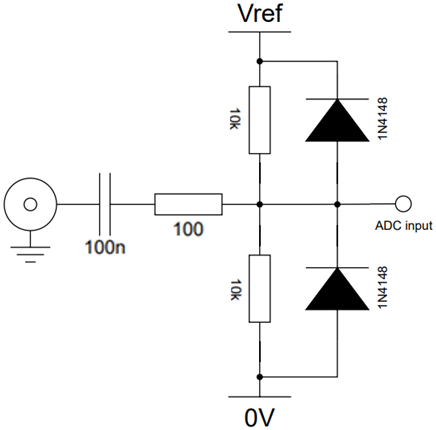
\includegraphics[width=0.4\textwidth]{adc_circuit.png}
   \caption{Circuit for line input into ADC}
   \label{fig:adccircuit}
\end{figure}

\pagebreak
Breaking the circuit down:
\begin{enumerate}
   \item Firstly, the audio line output signal is passed serially through a $100nF$ capacitor which acts as an open circuit for the DC component of the signal. Thereby, allowing only the AC component of the signal to pass.
   \item Secondly, a serial $100\Omega$ resistor is used to simply limit circuit current.
   \item At the first junction a voltage divider containing two $10K\Omega$ resistors is used \cite{VoltageDividerWiki}. Thus, halving the input voltage range spanning from $V_{ref}$ to ground and placing the signal within the suitable range for the ADC.
   \item A parallel second junction to the voltage divider of two respective $1N4148$ diodes is used to protect the circuit from overvoltage (falling outside the ADC range) \cite{1n4148-datasheet}. If one input exceeds the ADC range then the opposite polar diode will begin to conduct and negate the excess voltage.
   \item Finally an ADC-appropriate signal is achieved.
\end{enumerate}

\begin{figure}[!ht]
   \centering
   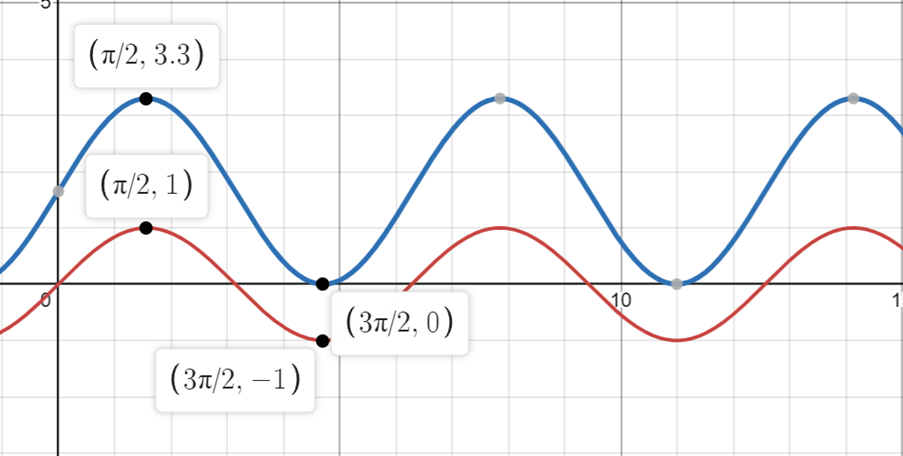
\includegraphics[width=0.4\textwidth]{LinetoADC.png}
   \caption{Line and ADC signals}
\end{figure}

In summary, the circuit described above serves as a conditioning stage for the audio signal before the signal is passed to the LPC4088 experiment board through the respective ADC input pin.
The analog signal is then sampled by the ADC and the obtained samples are converted into a digital value which can be read as scaled bits from memory.

% The values passed through the ADC input pin can then be read as scaled bits from the memory allocation indexed.
\vspace{1em}
\textbf{Implementation:}

\emph{Note: All additional hardware components were sourced by the Computer Engineer through the electronics supplier 'Fabian Enterprises Ltd'}

The issue faced and previously discussed is the need to convert the line level output received from the audio jack to a voltage level that can be read by the ADC.

On implementation of the required circuit, the listed components were acquired and the circuit was assembled following the schematic provided.
The circuit was tested with an oscilloscope to ensure that the output was being centered correctly between the $0$ and $V_{ref}$ levels.
Before trying to connect directly to the microcontroller, testing was done to ensure that no damage would be done to the microcontroller and the ADC components.

It should be noted that the initial implementation of the circuit indeed did not work fully as expected, due to one of the 1N4148 diodes being blown out.
This initially led to the belief that the diodes' orientation was incorrect.
However, after testing the diodes separately and replacing the blown diode, the circuit was tested again and the output was as expected.

\begin{figure}[!h]
   \centering
   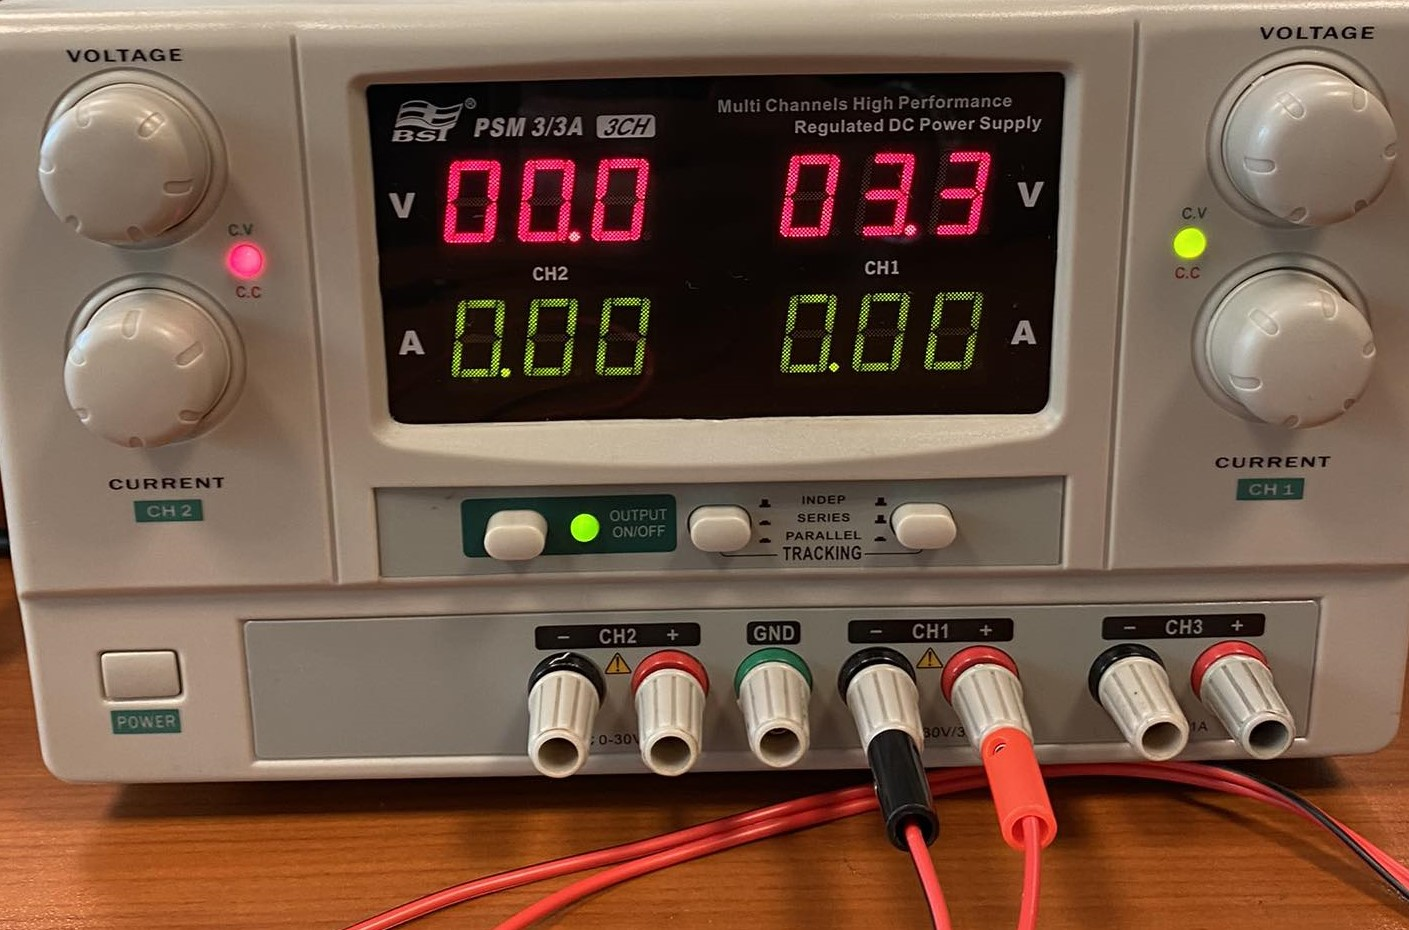
\includegraphics[width=0.8\linewidth]{vref.jpg}
   \caption{Voltage Supply set for $V_{ref}$}
   \label{fig:vrefvoltageexample}
\end{figure}

\vspace{1em}

\begin{figure}[!h]
   \centering
   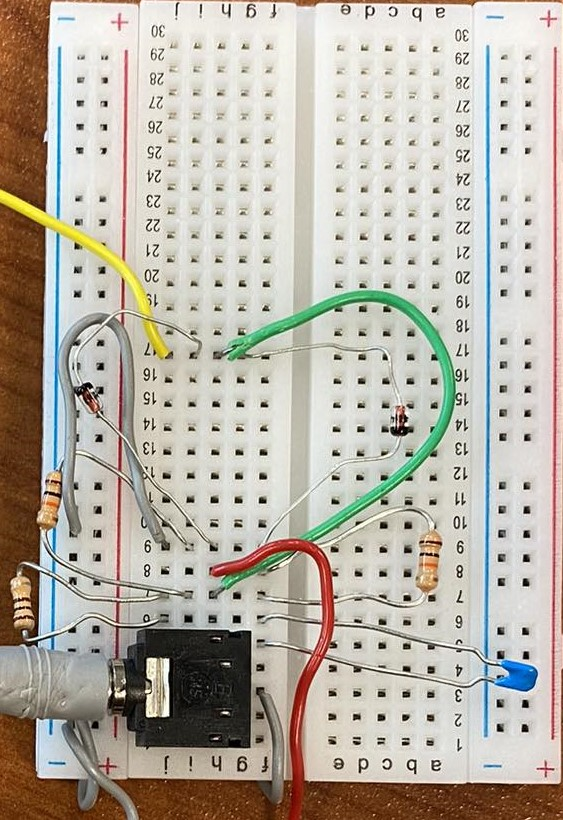
\includegraphics[width=0.8\linewidth]{circuit.jpg}
   \caption{Circuit Implementation}
   \label{fig:ciruitimplentation}
\end{figure}

\newpage

The output of a quiet region without the circuit connections can be seen in figure \ref*{fig:quietbeforecircuit}.
In the plot, the cursor indicates the required region that the output should be centered around.
However, it is clear that the output is not centered around the required region.

\vspace{1em}
\begin{figure}[!h]
   \centering
   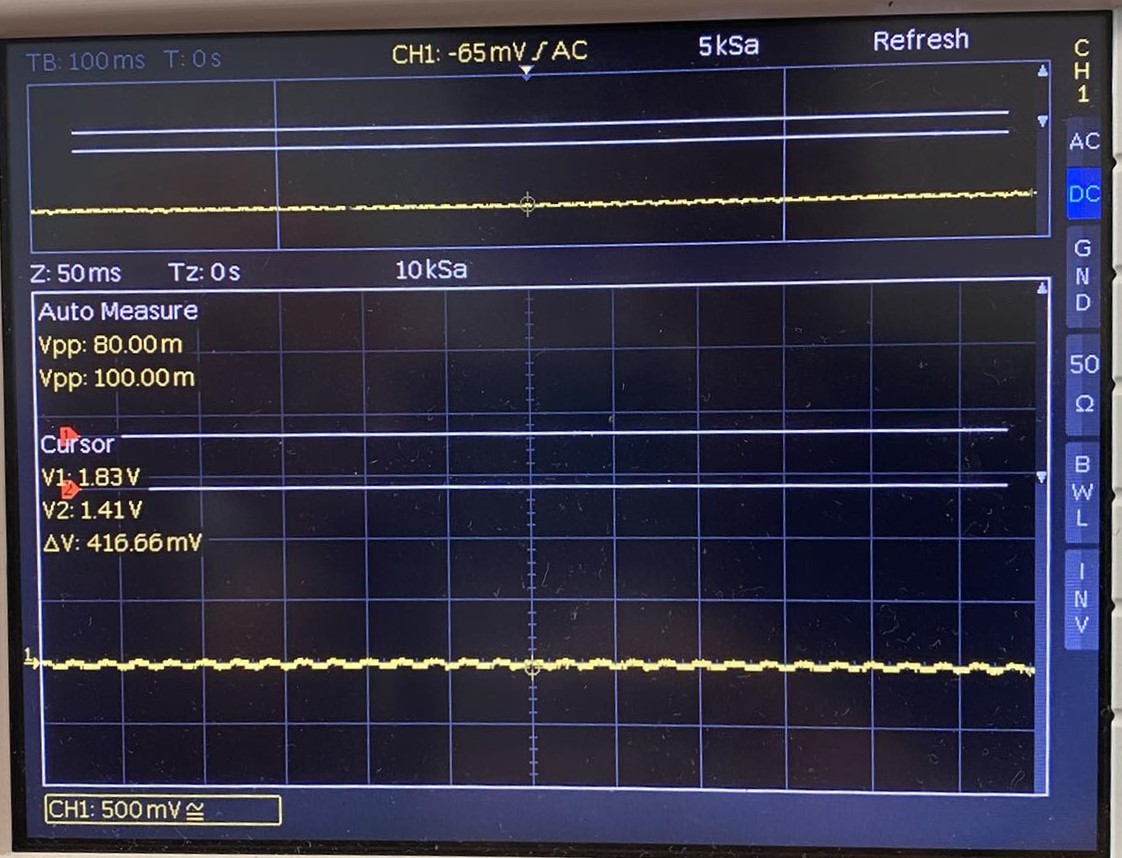
\includegraphics[width=0.8\linewidth]{shifted_difference.jpg}
   \caption{Quiet signal before circuit}
   \label{fig:quietbeforecircuit}
\end{figure}
\vspace{1em}

In figure \ref*{fig:quietaftercircuit} below, we can see the same quiet signal after being connected with the circuit.
The output is now centered around the required region ($1.6V$ or $\frac{V_{ref}}{2}$).
This indicates that the circuit is working as expected and thus the output signal should be able to be read by the ADC.

\vspace{1em}
\begin{figure}[!h]
   \centering
   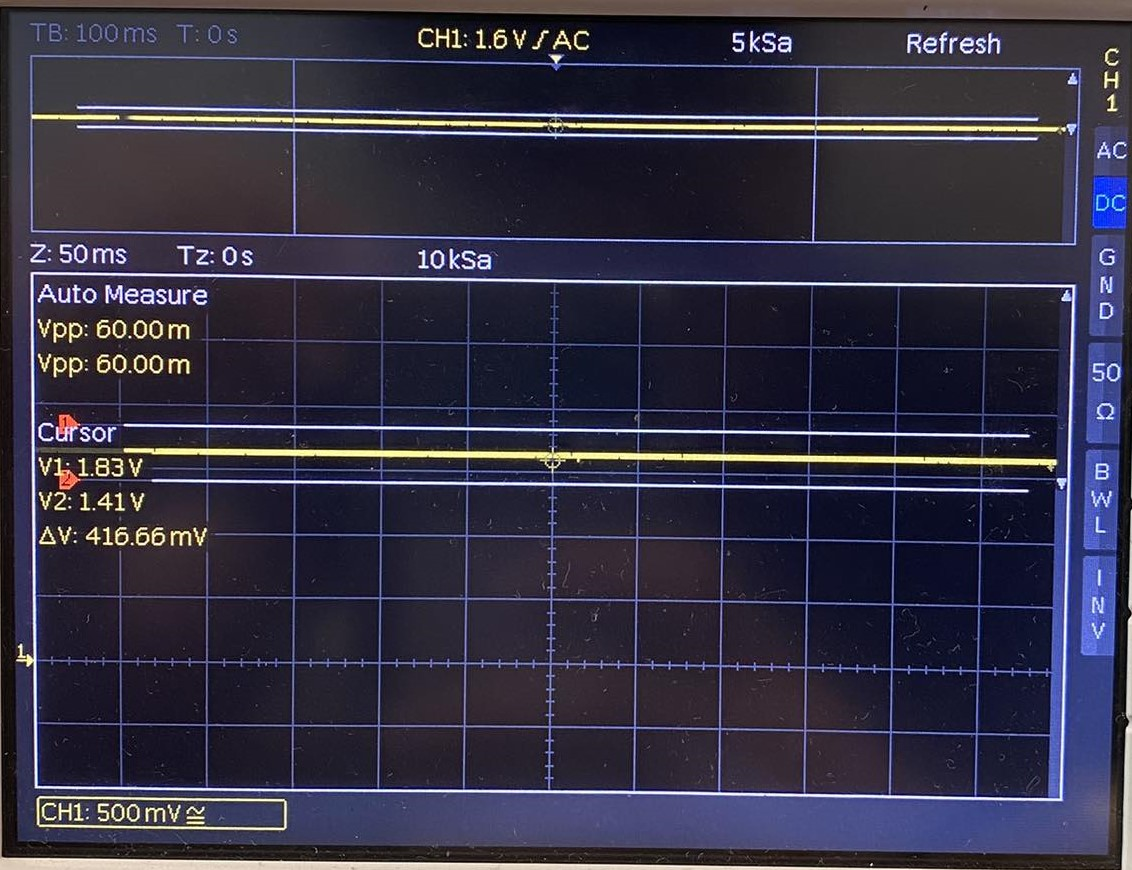
\includegraphics[width=0.8\linewidth]{quite_shifted.jpg}
   \caption{Quiet signal after circuit}
   \label{fig:quietaftercircuit}
\end{figure}
\vspace{1em}

In figure \ref*{fig:jacks}, the direct connection of the headphone jack output to the oscilloscope can be seen. This is done by identifying the left, right and ground connections of the headphone jack and connecting the respective oscilloscope probes to the ground and right/left connections. Knowing that the output is a stereo signal, the left and right channels were tested separately, but the results were the same.

\begin{figure}[!h]
   \centering
   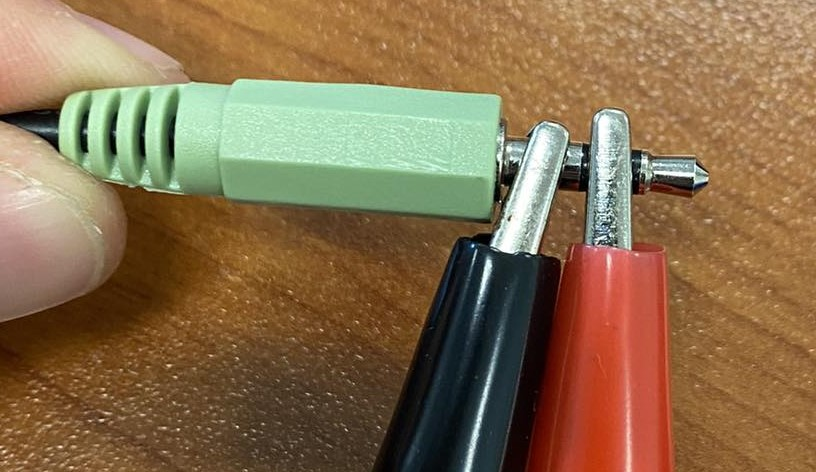
\includegraphics[width=0.8\linewidth]{jack_connections.jpg}
   \caption{Jack Connections}
   \label{fig:jacks}
\end{figure}

\newpage

In figure \ref*{fig:signalbeforecircuit}, the output of a signal being played directly from the headphone jack connection, shown in figure \ref{fig:jacks}, can be seen.
The output is not centered around the required region and the signal is not able to be read by the ADC.

\vspace{1em}
\begin{figure}[!h]
   \centering
   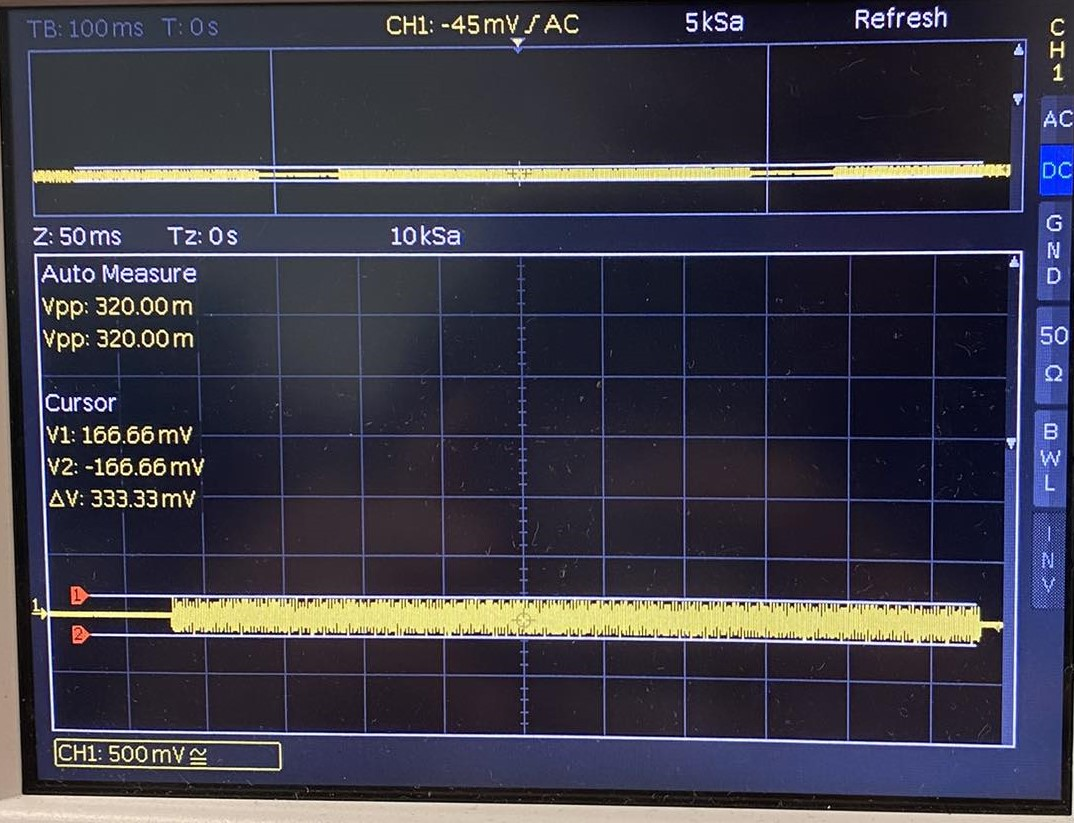
\includegraphics[width=0.8\linewidth]{signal_unshifted.jpg}
   \caption{Unshifted Signal}
   \label{fig:signalbeforecircuit}
\end{figure}
\vspace{1em}

In figure \ref*{fig:signalaftercircuit}, the output of a signal is now connected to the circuit.
In contrast, to figure \ref*{fig:signalbeforecircuit}, the output is now centered around the required region and the signal can be read by the ADC.
However, in both figures, it was noted that the signal power received is relatively low.
This is due to the audio player properties at the laptop output (even when the volume is set to the maximum).

A solution to this was to use a different source player such as an mp3 player or phone with a higher output power.
The implementation of an amplifier in the circuit was also discussed.
However, the ADC was still able to read the signal and the power was sufficient for the purposes of the project.
Therefore, the complication of adding an amplifier was not pursued.
This was an engineering decision made to keep the project simple and within scope.

\vspace{1em}
\begin{figure}[!h]
   \centering
   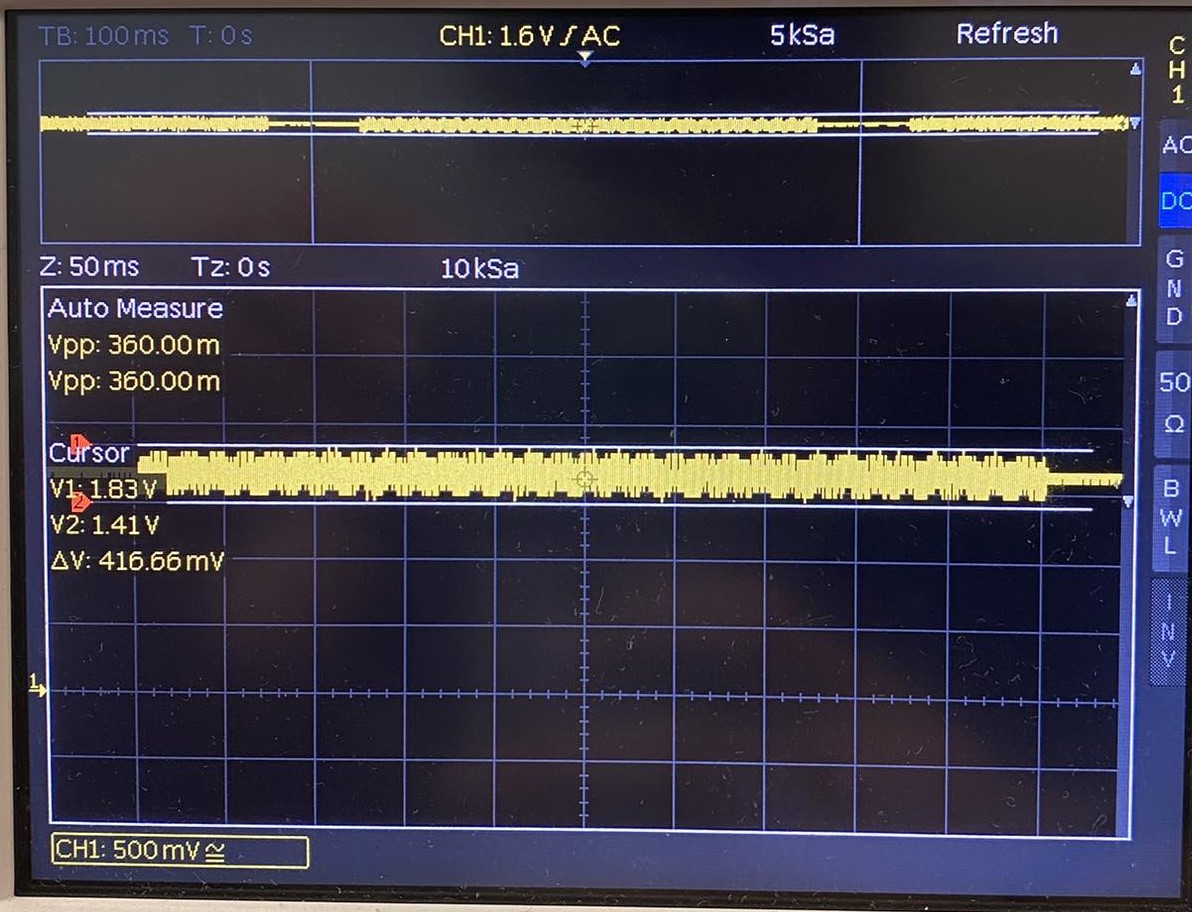
\includegraphics[width=0.8\linewidth]{signal_shifted.jpg}
   \caption{Shifted Signal}
   \label{fig:signalaftercircuit}
\end{figure}
\vspace{1em}

\newpage

From the provided LPC4088 board manuals, the respective pin configurations for $V_{out}$, which is our $V_{ref}$ is $3.3V$, ground, and the ADC input pins were identified.
The pins identified are highlighted in figure \ref*{fig:pinconfiguartions}.
The connections were made on the board as shown in figure \ref*{fig:onboardconnections} and the circuit was tested.
Having the ADC properly configured and the connections made, the ADC was able to read the signal and map it to the $12$ bits, $4096$ levels, of the ADC.
The digital signal value was then printed and observed accordingly for multiple tests.

\begin{figure}[!h]
   \centering
   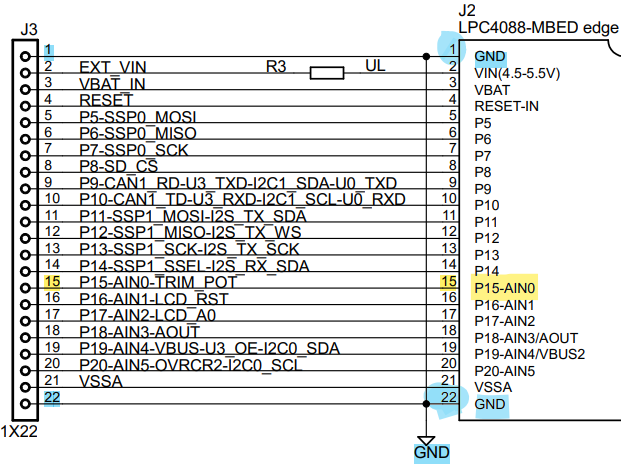
\includegraphics[width=0.95\linewidth]{pin_config_1.png}
   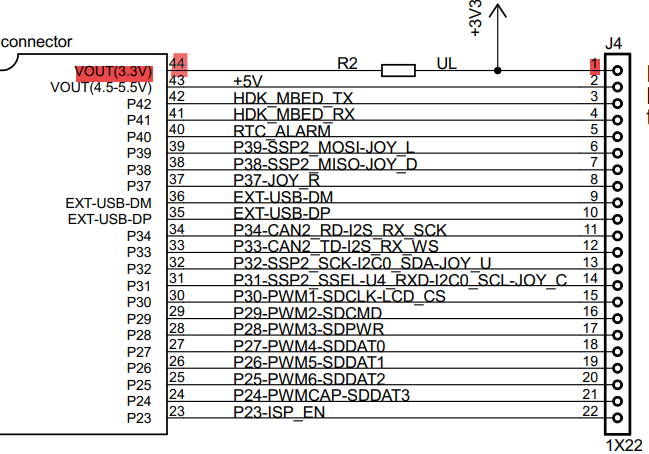
\includegraphics[width=0.95\linewidth]{pin_config_2.png}
   \caption{Pin Configuration}
   \label{fig:pinconfiguartions}
\end{figure}

\vspace{1em}

\begin{figure}[!h]
   \centering
   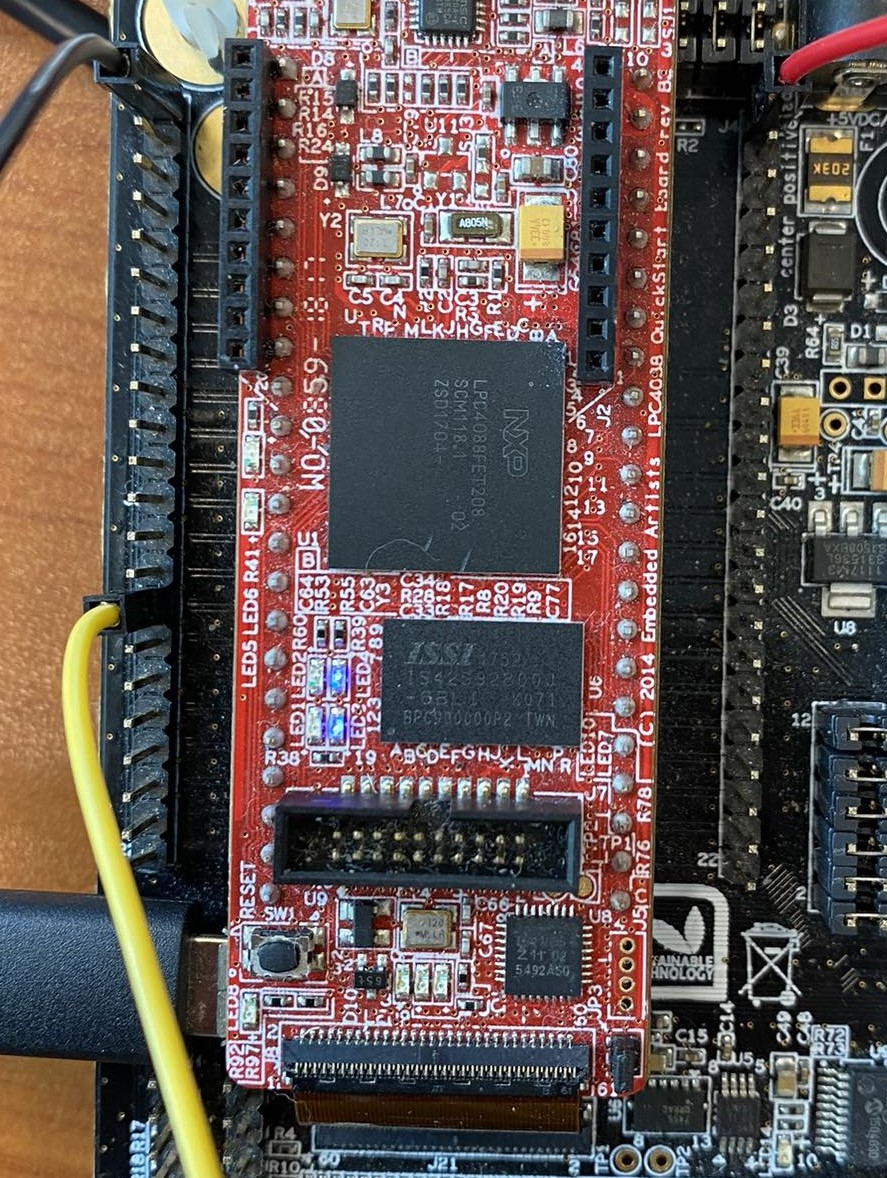
\includegraphics[width=0.7\linewidth]{board_connections.jpg}
   \caption{Onboard Connections}
   \label{fig:onboardconnections}
\end{figure}

\subsubsection{User Interaction Switch}
\textbf{Explanation:}

A switch will be used to facilitate user interaction with the system.
This includes modifying system settings to enable/disable scrolling, clearing the LCD, entering debugging mode, and shutting the system down.
This will be done through the GPIO pins which connect the switch to the LPC4088 microcontroller, which in turn monitors the state of the switch and takes appropriate actions based on user input.

\vspace{1em}
\textbf{Implementation:}

The switch input is read using the switch driver function \textit{switch\_get(PIN)} which returns the state of the switch position inputted as a parameter (\textit{SW\_UP, SW\_DN, SW\_LT, SW\_RT or SW\_CR}).
This function is called on every iteration within the main loop.
In the case of this project, all available switch positions have been used to trigger an operation.

\vspace{1em}
\textbf{The following are the respective operations for each switch position:}

\begin{itemize}
   \item[{}] \textbf{\underline{Switch UP:}} Toggles the auto-scroll flag, erases the previous value stored in the EEPROM and then writes the new value of the flag (which is 1-bit). The auto-scroll functionality manages how the LCD, displays the decoded output. When the flag is set to $0$, if the display is full, the screen is cleared and the next decoded result will be outputted at the top-left position on the LCD. On the other hand, when the flag is set to $1$, if the display is full, the last row is shifted up and the next decoded result is outputted at the start of the second row. When auto-scroll is enabled the LED emits a blue light unless the system is in the debugging mode (reading ADC value) where a constant white light indication must be seen.
      \vspace{0.5em}
   \item[{}] \textbf{\underline{Switch CENTRE:}} Clears the LCD screen. This LCD clear function is called and the cursor position is resetted. The LED also emits a green light to indicate that the LCD has been cleared.
      \vspace{0.5em}
   \item[{}] \textbf{\underline{Switch DOWN:}} Terminates the program. The switch down clears the LCD, displays a "Goodbye" message on the LCD and exits the program. The system may be restarted through the reset button to rerun the flashed program.
      \vspace{0.5em}
   \item[{}] \textbf{\underline{Switch RIGHT:}} Terminates the program. Same implementation as switch DOWN.
      \vspace{0.5em}
   \item[{}] \textbf{\underline{Switch LEFT:}} Toggles the debug mode flag to enter a debugging state for the potentiometer value. ADC readings are affected by the onboard hardwired potentiometer, therefore, a respective interface to be able to see the effect of the potentiometer is present. The LED emits a white light in order to indicate that the system is in debug mode and the cursor position is reset before displaying the ADC values.
\end{itemize}

On each iteration within the main function, a sequence of if statements is employed to identify which switch position has been triggered and thus perform the respective operations.
It is to be noted that since the switch holds its state for longer than one reading per human switch toggle, the logic was built to only read on the rising edge ($0 \rightarrow 1$) or the falling edge ($1 \rightarrow 0$).
This was handled using flags that hold the previous switch state and comparing them to the current read value before executing the switch operations.

\subsubsection{Liquid-crystal display}
\textbf{Explanation:}

The Hitachi HD44780-based 16x2 LCD is interfaced with the LPC4088 microcontroller using GPIO pins for data signals, control signals, and power connections (VCC and GND) \cite{hd44780-datasheet}.
The microcontroller will send commands and data to the LCD in order to display the decoded output to the user.

\textbf{Implementation:}

The LCD driver and its functions are used to display output to the HD44780. An unsigned short int was used to keep track of the cursor position on the 16 X 2 display. The initialization and use of the driver functions are done in the main file.

\vspace{1em}
\textbf{The following are the features added to the LCD:}

\begin{itemize}
   \item[{}] \textbf{\underline{Automatic Scrolling:}} This makes use of LCD functions to clear the LCD screen, the functions to print, and the functions to move the cursor. By default, the system is set up so that it always stores the output in the second row of the LCD. When auto-scroll is toggled on, the system will clear the screen, print the previous second row stored, and move the cursor to the first line in the second row. This allows the system to display the output in a continuous manner.
      \vspace{0.5em}
   \item[{}] \textbf{\underline{Welcome Message:}} Another feature added to the LCD is the start message which is defined in the \textit{printStartMessage} function. Here a pointer to a string of characters holding the message to be displayed is passed as a parameter. Using the LCD driver functions, the LCD is first cleared, then the message passed as a parameter is printed and after a delay, the LCD is cleared again.
      \vspace{0.5em}
   \item[{}] \textbf{\underline{Debug Mode:}} When debug mode is toggled on, the ADC values are displayed on the LCD. This is done by resetting the cursor position and then printing the ADC values to the LCD. The ADC values are displayed after a sequence of 25 filled buffers. This is done to slow down the intervals of displaying to the LCD without slowing the actual system itself from running normally. This makes the ADC values more legible to the human user.
\end{itemize}

\subsubsection{Feedback LED}
\textbf{Explanation:}

The onboard RGB LED is used to provide visual user feedback on the system state. The LED emits different colors based on the system state, such as red for an error state, green after clearing the LCD, blue for auto-scrolling and white for debug mode. The LED is controlled using the GPIO pins of the LPC4088 microcontroller.

\vspace{1em}
\textbf{Implementation:}

The feedback LED is a component found on the LPC4088 board and is hardwired. The LED driver is used to initialize the functionality as well as to set the respective color that needs to be displayed. The \textit{leds\_set} function accepts $3$ integer parameters that correspond to the different colors red, green, and blue. If a $0$ is passed as a parameter, then that color is not emitted, however, if a number greater than $0$ is passed as a parameter then the corresponding color is emitted. Lastly, if more than one of the colors are passed $1$ as a parameter then a mix of the two colors will be emitted.

\vspace{1em}
\textbf{The following is the meaning assigned to each color:}

\begin{itemize}
   \item[{}] \textbf{\underline{No Light:}} If no light is being emitted from the LED, it indicates that the system is performing in the default decoding state without any flags set, that is, the system does not have auto-scroll enabled nor is it in debug mode.

   \item[{}] \textbf{\underline{Blue Light:}} As previously mentioned, the blue light indication on the LED shows that auto-scroll is enabled. This light is useful for debugging the EEPROM, this is because one can visually see the auto-scroll flag being toggled back on after the system is restarted.

   \item[{}] \textbf{\underline{Green Light:}} The green LED indication is flashed when the user clears the screen by pressing the switch's centre. This light is valuable information to visualize that the input to clear the LCD has been received.

   \item[{}] \textbf{\underline{Red Light:}} The red LED indication is used in the case when an error state has been detected. The LED will flash red when the system detects two high or low frequencies.

   \item[{}] \textbf{\underline{White Light:}} The white light indicates that the user has entered debugging mode. Here the user can view the ADC value change while adjusting the potentiometer. The LED keeps emitting white light until the user exits this state.
\end{itemize}

For switching between LED colors the debug mode and auto-scroll flags are used as parameters in the \textit{leds\_set} function. This function is called during state switches and after every decode to ensure that the right led indication is indicated at all times.

\newpage

\subsection{Interrupt-Driven Sampling}
\textbf{Explanation:}

The system is designed to be multithreaded by emulating two threads, a sample thread and a main thread. This is done through the use of a timer that calls an interrupt handler at a frequency of $8000Hz$. The interrupt handler triggers the ADC to sample the input signal. The sample rate was chosen based on the Nyquist theorem, which states that the rate should be at least twice the highest frequency of the signal, for accurate measurement.

The reason a frequency of $8000Hz$ was chosen over simply tripling the result of the lowest + highest frequencies was due to this paper \cite{DTMF_Frequency_Choice}.

\vspace{1em}
\textbf{Implementation:}

\textbf{\underline{Timer:}} The timer is set up through the function \textit{startSamplingTimer}. The function first initializes the timer using the timer driver function \textit{timer\_init} which triggers an interrupt at a frequency of $8000Hz$ by passing the clock rate of the microcontroller ($120MHz$) divided by the desired frequency ($8000Hz$) as a parameter. Next, the \textit{timer\_set\_callback} function is used to choose which function is called as an interrupt handler, in this case, \textit{samplingInterrupt}. The timer is then started using the \textit{timer\_enable} function.

\vspace{0.5em}

\textbf{\underline{Interrupt Handler:}} The interrupt handler function is set up by creating the function \textit{samplingInterrupt}. The function reads the ADC value using the ADC driver function \textit{adc\_read} and then stores the ADC value obtained in a buffer. It also handles the switching of buffers for double buffering.

\subsection{Double buffering}
\textbf{Explanation:}

The system is designed to store the ADC samples in a buffer. To make sure that the system has enough time to decode the signal and simultaneously does not miss any samples, two buffers are used. The system alternates between the two buffers, allowing one buffer to be filled while the other is being decoded.

\vspace{1em}
\textbf{Implementation:}

This is done by creating two buffers as well as a pointer to indicate which buffer is currently being filled. Within the interrupt handler, using an if statement, we check if the current buffer being filled is full and if so, the pointer is changed to point to the other buffer. The system then within the main loop decodes the filled buffer while the other buffer is being filled.

\subsection{Decoding using the Goertzel Algorithm}

The system is designed to use the Goertzel algorithm when processing the samples within the buffer.
This algorithm was chosen for this because it is more computationally efficient when it comes to detecting already known tones.
Each time a buffer is filled, the Goertzel algorithm is run over the entire buffer eight times, once for each frequency, and the two highest results determine the tone mapping to be printed.

The algorithm was first attempted in Python, and then later implemented in C.
The jupyter-notebook found within the test folder called \textit{goertzel-test.ipynb} was presented to the group during a meeting to agree on using the Goertzel algorithm over a Fast Fourier Transform implementation.
The notebook contains a general idea of how the C implementation is made.

\subsubsection{Decoding function}

Decoding is done through the function \textit{processSample} which takes a pointer to the current buffer and a frequency of interest.

The function returns the power term for the frequency of interest.
This means that the higher the power term, the more likely the frequency of interest is part of the input signal.

Within the function \textit{decode}, \textit{processSample} is called eight times and the low and high frequencies with the highest powers are saved.

\subsubsection{Tone Mapping}

From the function \textit{decode}, after the two highest powers are saved,
they are passed to the function \textit{toneDetection}.

This loops through a constant array to find the corresponding DTMF character and return it or return $\textbackslash0$ in the case that no mapping is found.

This character is then returned from \textit{decode} to the main loop of the program for printing.

\subsubsection{Buffer Size}

According to the DTMF standard in ITU-T recommendation Q24 \cite{itutrecommendation24}, following the AT\&T standard, the pause duration (time between tones) and signal duration (duration for which a signal is valid) are to be $40ms$ at minimum.

To achieve this, following the below formula, at $8000Hz$ we would need $320$ samples for $40ms$.

$$
   \text{Samples} = \text{Frequency} \times \text{Time}
$$

To ensure that we were able to measure tones at a rate of $40ms$ we chose to measure tones at a slightly faster rate of $30ms$.

Thus, a buffer size of $240$ samples was chosen, meaning both tones and pauses at $30ms$ minimum can be detected.

\subsubsection{Tone Detection}

Following the same paper as above \cite{itutrecommendation24},
a threshold of $1.5\%$ was the aim when detecting tones. This means that for frequency $697Hz$ we should accept $\pm10Hz$. Whilst for frequency $1633Hz$ we should accept $\pm25Hz$.

Our system was unable to properly accept the high frequencies at $\pm25Hz$ so we chose to lower it to $\pm13Hz$.

The constant \textit{GOERZTEL\_THRESHOLD} represents $2$ below the value of $697\pm10Hz$ and $1633\pm25Hz$. This constant was chosen from testing with a frequency generator app by LuxDeLux on the Android PlayStore \cite{FrequencyGeneratorApp}. Tests were done by measuring the value of \textit{processSample} for each frequency. The result was that a value of $125$ was chosen for \textit{GOERZTEL\_THRESHOLD}.

\textbf{Note:} Our system has a limitation as it operates effectively only at high volume levels due to its threshold setting.
It is possible to manually lower this threshold, for example, to $65$, but this adjustment reduces the required volume.

To clarify, the system functions optimally within a specific volume range determined by the threshold setting.
For instance, with a threshold of $125$, the system operates at $100\%$ efficiency for inputs with an amplitude of $1$ and within the range of $-6dB$ to $0dB$. While it may function with other settings, it is not guaranteed.

Lastly, this limitation could have been fixed with further tinkering to normalize the input buffer and adjust the threshold dynamically.
However, these solutions were not implemented due to the inability to find a reliable version.

\subsubsection{Quiet Detection}

To avoid running the algorithm when there is no tone within the signal,
the function \textit{quietDetection} is run before any processing is done.
This function takes the absolute sum over all the samples within a buffer and compares that to a constant \textit{QUIET\_THRESHOLD}.

This constant was chosen from repeated testing. Briefly, these were the steps taken to determine the value of \textit{QUIET\_THRESHOLD}:
\begin{itemize}
   \item The volume for a computer was set in increments of $10$ from $10$ till $100\%$ volume.
   \item A measurement was taken for the idle quietness.
   \item Another measurement was taken while a constant tone was being played.
\end{itemize}

Results:
\begin{itemize}
   \item Idle sum was constant $0.85$ throughout.
   \item Tone sum ranged from $2.0$ at $10\%$ to $84.6$ at $100\%$
\end{itemize}

Thus, the value of $1.5$ was chosen for \textit{QUIET\_THRESHOLD}.

\subsubsection{Optimizations}

Within the decoding function, \textit{processSample}, the $2*cos\theta$ in the Goertzel algorithm is pre-calculated and stored in memory for every frequency.
This avoids extra computation as the value is static as long as we use an $8000Hz$ sampling rate.

\subsection{EEPROM and Persistent Memory}

For this project, it was decided that the state of the auto-scroll flag is to be stored and persisted when the program is restarted.
Since the auto-scroll flag is simply an unsigned char the EEPROM simply needs to store the byte flag.

In the ARM Cortex M4, there are two methods of persistent storage; flash and EEPROM.
Flash is a non-volatile memory that can be written to, however, it has a limited number of write cycles.
EEPROM is a non-volatile memory that can be written to as well, however, it has a much higher number of write cycles.
Therefore, the EEPROM is chosen as the persistent storage method for the project.

Consequently, an EEPROM driver is required.
The EEPROM driver is sourced from the NXP MCU SW Application Team and modified for the project specifications.
The driver functions include the initialization function \textit{eeprom\_init}, the write function \textit{eeprom\_write}, the read function \textit{eeprom\_read} and the erase function \textit{eeprom\_erase}.

\subsubsection{EEPROM Initialization}

The EEPROM initialization function is used to initialize the EEPROM driver.
The function is called at the start of the program to ensure that the driver works in divisions of the main system clock and to set the respective wait states for the EEPROM.

\subsubsection{EEPROM Read}

The EEPROM read function is used to read the flag value at the chosen address where it is stored.
The function takes four parameters the EEPROM page offset, the page address, the pointer to the data to be read into and the length of the data to be read.

The function begins by clearing the interrupt flag and setting the respective page address and offsets of the EEPROM to be read from.
The EEPROM is set into read mode and an iterative loop is used to read the data into the pointer.
The loop consists of waits for the EEPROM status to be ready from the read and a page overflow check.
Note since we are only reading a byte from a given page the page overflow check should never be triggered, but is included for completeness of the driver.
We are also only reading in the 8-bit mode of the EEPROM.
However, it is capable of also reading in 16-bit and 32-bit modes.
The function then returns the data read into the pointer and the auto-scroll flag is read and set accordingly in the main program.

\subsubsection{EEPROM Write}

The EEPROM write function is used to write the auto-scroll flag value to the chosen address when updated.
The function takes the same four parameters as the read function.

The function begins and functions very similarly to the read function.
It begins by clearing the interrupt flag and setting the respective page address and offsets of the EEPROM to be written to.
The EEPROM is set into write mode and an iterative loop is used to write the data from the pointer.
The loop consists of waits for the EEPROM status to be ready from the write and a page overflow check.
Once again since we are only writing in the 8-bit mode and only a byte is to be written, the page overflow check should never be triggered.

The function then sets the interrupt flag to wait for the end of the program, sets the respective address page written to at the end and erases the program page to ensure that only the data written is stored and done so correctly.
The function waits till the end of the program and does not need to return any data.

\subsubsection{EEPROM Erase}

The EEPROM erase function is used to erase data at the chosen address.
The erase function is essential in EEPROM logic to ensure that the data written is the only data stored in the address.
This function will preceed the write function.

The function takes the page address to be erased as a parameter and begins by setting the interrupt flag to wait for the end of the program, it then sets the respective address page to be erased.
The function works by writing zero to the data in the page address.
The function then waits till the end of the program and does not need to return any data.

\subsection{Debug Mode (ADC Potentiometer Adjustment)}

Due to the onboard hardwired potentiometer, the read ADC values can be inaccurate, if not adjusted correctly.
The resistance effect will cause the signal to be read differently and even not read, due to the fact that the values of frequencies are calculated off of the ADC amplitude scaling voltage values.

As a result, a state in which the user is able to negate this effect by setting the potentiometer to a valid state where its effect will not be felt is created.
As discussed before, to enter this state the user must press the switch to the left.
In order to exit and continue decoding normally the user must press the switch to the left again.

Once in debug mode, the LED emits white light and the user will enter a state in which the value of the ADC is constantly printed.
This value should be set to as accurately zero as possible.
It is crucial that when setting the ADC potentiometer, no signal is being played to the system so that an ADC value of zero is true to the signal power.

The ADC values being printed on the LCD were initially seen to flicker and update too quickly to be properly legible for the human user.
Therefore a delay separate from the system clock is added in order to slow down the intervals of displaying to LCD without slowing the actual system itself from running normally.
This delay is a simple counter that enters the if statement when both the ADC flag is on and the counter is zero.
The counter counts to $25$ and is then set back to $0$ essentially delaying the displays to one every $25$ filled buffers.
While displaying ADC values, we still keep storing the ADC values in the buffer so that we may return to decoding as before.

This implementation was a method of overcoming an issue faced during the implementation of the system.
However, it serves to offer valuable information for debugging purposes and about the functionality of the system.

\subsection{Error State}

The error condition identified in the system is the case when two high frequencies or two low frequencies are detected by the system.
The DTMF decoder will still decode these signals being a Fourier transform function but the process will simply not be able to identify the signal.
When this is the case, a '!' symbol is generated and the system will output it in the same position as if it was decoded correctly.
The error state is also indicated by the LED flashing red.

As previously mentioned, when an error state of such nature occurs the program will not halt as the DTMF decoder still processes the frequencies.
Therefore, following an error, the system will continue to decode normally.

% Note when such an error is encountered, depending on how the signal is passed there might be some missed DTMF codes. That is if a DTMF signal is played in sequence with a high/low frequency producing signal. The DTMF signals at which the second signal also occurs will be missed.

\subsection{Functional Requirements}

\begin{description}
   \item[\parbox{0.5\textwidth}{\underline{Requirement 1:} Solution must be real-time; reacting to one or more inputs that can change at any time.\vspace{2mm}}] \underline{Description:} The system constantly samples input signals, allows the user to clear display, and toggle configurations using the switch. Using the ARM MDK, sampling is done through a timer, whilst, the switch input detection is done through constant checks in the main loop. In this way, the system can react to real time inputs.
   \item[\parbox{0.5\textwidth}{\underline{Requirement 2:} System must make use of at least one digital input.\vspace{2mm}}] \underline{Description:} The system contains a switch with multiple functionalities. A centre press clears the LCD display, a toggle-up enables/disables auto-scrolling, a toggle-left enables/disables debug mode, and a press down or right terminates the program. Using the MDK this is achieved using the GPIO drivers which facilitate configuring and using inputs such as switches.
   \item[\parbox{0.5\textwidth}{\underline{Requirement 3:} System must make use of at least one digital output.\vspace{2mm}}] \underline{Description:} The system makes use of the onboard RGB LED to provide immediate visual feedback of the system status. This is done through the MDK's GPIO drivers which provide control to the LED's on and off state.
   \item[\parbox{0.5\textwidth}{\underline{Requirement 4:} System must connect to at least one external peripheral.\vspace{2mm}}] \underline{Description:} A Hitachi HD44780-based 16x2 LCD display is used to output the decoded result. This can be achieved through manipulating GPIO pins to communicate with the LCD. These are pin P1\mathunderscore24 (used for serial data input), pin P1\mathunderscore20 (acts as the clock signal for synchronizing data transmission) and pin P1\mathunderscore2 (signals the transfer of data from the shift register to the output latches).
   \item[\parbox{0.5\textwidth}{\underline{Requirement 5:} On power up or reset, system should enter a well‐defined safe state.\vspace{2mm}}] \underline{Description:} Using the MDK, the system is designed to only respond to valid inputs, thus the system will never enter an undefined state.
   \item[\parbox{0.5\textwidth}{\underline{Requirement 6:} System must persistently store configuration settings, independent of the position of physical switches.\vspace{2mm}}] \underline{Description:} The ARM MDK supports interfacing with non-volatile memory devices such as flash memory and EEPROMs. The EEPROM is used to persist the auto-scroll flag state such that when the system is restarted the previous auto-scroll flag state is automatically set.
   \item[\parbox{0.5\textwidth}{\underline{Requirement 7:} System shall have a useful and appropriate mechanism for indicating error conditions to the user.\vspace{2mm}}] \underline{Description:} As mentioned previously, using the MDK the LED will emit a flash of red light to indicate that the system has encountered an error, and an '!' is outputted instead of the decoded result.
   \item[\parbox{0.5\textwidth}{\underline{Requirement 8:} System should be robust (incorrect input is handled)\vspace{2mm}}] \underline{Description:} In the event of incorrect input, the system will ignore the input without performing any action, ensuring that it remains in a stable and expected state.
\end{description}

\subsection{Software Partitioning}

\begin{itemize}
   \item[{}]\textbf{\underline{src/main.c:}} Main runner file which contains the main loop of the program. This file is responsible for initializing the system, sampling signals, detecting switch input, manipulating the LCD and making use of the decode and EEPROM functions.
   \item[{}]\textbf{\underline{include/eeprom.h:}} This header file declares the functions and constants required for EEPROM operations.
   \item[{}]\textbf{\underline{include/decode.h:}} This header file declares the functions and structures required for the Goertzel algorithm.
   \item[{}]\textbf{\underline{src/eeprom.c:}} This file implements the EEPROM functions, which include; initialization, reading, erasing and writing.
   \item[{}]\textbf{\underline{src/decode.c:}} This file implements the functions required for the Goertzel algorithm.
\end{itemize}

\section{Management}

\subsection{Time Plan and Dependencies}
\vspace{1em}
We identified 9 tasks that needed to be tackled.
These tasks can be seen in the legend on the left-hand side of the Gantt Chart\cite{GANTT_Wikipedia} figure (Fig \ref*{figure:ganttChart}).

\begin{figure}[!h]
   \centering
   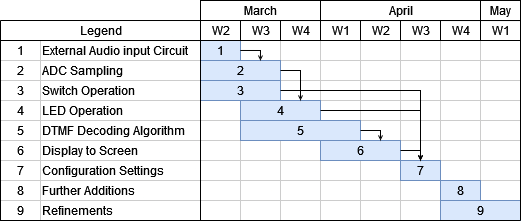
\includegraphics[width=0.45\textwidth]{GanttChart.png}
   \caption{Gantt Chart showing our proposed time plan}
   \label{figure:ganttChart}
\end{figure}
\vspace{1em}
The required responsibilities were assigned among the members of the group. Below is a breakdown of our individual assignments:
\begin{enumerate}
   \item Graham Pellegrini was assigned: Primarily the External Audio Input Circuit, Secondarily Configuration Settings (EEPROM), and Thirdly Decoding.
   \item Luca Vella was assigned: Primarily Decoding, Secondarily LED Operation, Thirdly Error Condition, \textbf{EXTRA:} Debug Mode
   \item Matthew Mifsud was assigned: Primarily ADC Sampling, Secondarily LCD Display Features, Thirdly Switch Operation.
   \item Julian Falzon was assigned: Primarily the Decoding Algorithm, Secondarily Configuration Settings.
\end{enumerate}

By 'Further Additions' we are referring to the implementation of any extra features that are not crucial to the functionality of the core DTMF decoder.
On the other hand, by 'Refinements' we mean optimization and refactoring of the code.
Thus, there was no particular individual assigned to these tasks.

It should be noted that the tasks in the chart were chosen to have a one or two-week deadline, with the decoding algorithm taking three weeks, depending on the complexity of the task.

The tasks in the chart are staggered such that they partially depend on the tasks above.
The arrows within the chart illustrate which parts require full functionality of a particular task before being able to move forward.
For example, a portion of task 2 depends on task 1, this could be the testing of whether input can be read.

\subsection{Development Model}

The Rapid Software Development model was selected for this project.
This model involves dividing the project into smaller, manageable parts that can be developed and tested in brief, iterative cycles.
Thus emphasizing speedy development, which was a fitting choice since some decisions changed and evolved \cite{RapidDev}.

\section{Video Demo}

The final working solution can be seen through a video demo found from this link: \url{https://drive.google.com/file/d/1tX34IHPbXN6ED1rxoBW5u12FEKO-R7fX/view?usp=sharing}

The demo goes through the setup of the input circuit, instructions on how to compile and load the project, and a demonstration of how to use the system and its features.

\section{Closure}

In conclusion, this design brief has outlined the challenges that were planned to be tackled as well as their corresponding solutions to meet all requested requirements.
The system was completed fully according to the requirements and the system was tested to ensure that it is functioning as expected.

\bibliographystyle{ieeetr}
\bibliography{references}

\end{document}